\section{Sistema Nervioso}

Conocer los pricipales componentes del sistema nervioso es esencial para el desarrollo de una RNA por varias razones:
\begin{itemize}
 \item Inspiración biológica:
    \begin{itemize}
    \item Nuestro sistema nervioso ha evolucionado para procesar información de manera eficiente, comprender sus componentes proporciona ideas valiosas para diseñar algoritmos y arquitectura de redes neuronales. 
    \end{itemize}
 \item Arquitectura y función:
    \begin{itemize}
    \item Comprender someramente la arquitectura y funciones del sistema nervioso en nuestro cuerpo, nos ayuda en la creación de modelos de redes artificiales que pueden realizar tareas específicas, como reconocimiento de patrones, procesamiento de lenguaje natural, y más.
    \end{itemize} 
 \item Aprendizaje y Adaptación:
    \begin{itemize}
    \item El sistema nervioso es capaz de aprender y adaptarse a través de experiencias. Conocer los mecanismos de aprendizaje en el cerebro puede inspirar algoritmos de aprendizaje profundo que permitan a las RNAs a mejorar su rendimiento con el tiempo.
    \end{itemize}
 \item Optimización de Rendimiento:
    \begin{itemize}
    \item El sistema nervioso está altamente interconectado, permite la comunicación rápida y eficaz entre las célular nerviosas. Esto nos guia en el diseño de conexiones eficientes en las RNAs para optimizar el rendimiento la transmición de información.
    \end{itemize}
 \item Robustez y tolerancia a fallos:
    \begin{itemize}
    \item El sistema nervioso es robusto y capaz de funcionar en condiciones adversas. La observación cuidadosa de esta capacidad, nos sugire estrategias para mejorar la robustez y la tolerancia a fallos en las RNA.
    \end{itemize}
 \item Ética y Seguridad:
    \begin{itemize}
    \item Al notar la gran complejidad de nuestro sistema nervioso, notamos también nuestros limites de imitación y semejanza que realmente se puede lograr. La responsabilidad de crear RNAs conlleva sus posibles riesgos y dilemas/desafíos éticos. 
    \end{itemize}
\end{itemize}


El sistema nervioso se estudia principalmente en dos partes, sistema nervioso periférico (SNP) y sistema nervioso central (SNC). El SNC es donde nos enfocaremos, este se compone principalmente por la medula espinal y el encéfalo que son los centros principales donde ocurre la correlación e integración de la información nerviosa. Es en el encéfalo donde se encuentra principalmente el cerebro, cerebelo y el tallo encefálico.\parencite{sistNerv}   

Un nervio es una estructura conductora de impulsos nerviosos.
Esta compuesto por una colección de axones los cuales son prolongaciones largas y delgadas de las células nerviosas agrupados en fibras y rodeados de vasos sanguíneos.
% Los axones, transmiten señales eléctricas y químicas entre las células nerviosas, forman una especie de "cable" a través del cual viajan los impulsos nerviosos. 
 Se origina desde la médula espinal o el encéfalo. %(31 pares de nervios raquídeos) o el encéfalo (12 pares de nervios craneales).

Los nervios en conjunto son la escrutura organizada por tejido conectivo en el sistema nervioso, encargada de transmitir información entre diferentes partes del cuerpo del SNP y del SNC, permitiendo así el control y coordinación eficientes de las actividades corporales. Se extienden desde el cráneo y la médula espinal para abarcar todo el cuerpo humano. \parencite{princNS5}

Los nervios del SNP se pueden clasificar en tres catergorias:

\begin{itemize}
\item \textbf{Nervios motores:} están asociados con las salidas y la ejecución de acciones, conectándose y ejerciendo su influencia sobre los músculos.
\item \textbf{Nervios sensitivos:} estos reciben señales de entrada, como en ojos, oídos y piel. Son responsables de transmitir información sensorial hacia el sistema nervioso.
\item \textbf{Nervios mixtos:} estos tienen tanto fibras sensitivas como motoras. Es decir, cumplen funciones tanto de entrada como de salida de información.
\end{itemize}

El SNC está compuesto por gran cantidad de células nerviosas excitables y sus prolongaciones, denominadas neuronas. \parencite{sistNerv}   %pag2 


\subsection{Cerebro}

Desde la parte tangible del cerebro hasta la intangible del pensamiento, está directamente relacionada con la forma que funciona nuestro pensamiento y reacciones motoras.


El cerebro, por su gran tamaño, da lugar a un mejor registro de su actividad. Los muchos registros realizados muestran que se incrementa la circulación de la sangre en el área del cerebro con mayor actividad neuronal. Se tienen identificadas regiones que se activan ante cierto estímulo. \parencite{neurona_A_cerebro}


 Se detecta cuánta sangre se está bombeando en diferentes regiones del cerebro dependiendo de los estímulos que se le presentan a una persona; o si alguna persona tiene un padecimiento, se toman escaneos para ver qué regiones del cerebro están funcionando y cuáles presentan lesiones. A partir de las lesiones y de la identificación de la actividad que ya no se puede realizar de forma normal, se infiere qué región era responsable de esa actividad que ahora está dañada.\parencite{estudiosF}

Para obtener más detalle de los estudios de la actividad del cerebro, ver el documental "The Brain with David Eagleman".

\subsection{Zonas funcionales}

En el cerebro, las diversas zonas identificadas con funciones específicas, están conectadas, por una ruta que se conoce como 
 ''la ruta desde la sensación hasta la cognición'' notemos un diagrama de la parte funcional del cerebro. \parencite{sensAcogn}
 


 \begin{figure}[h]
  \centering
  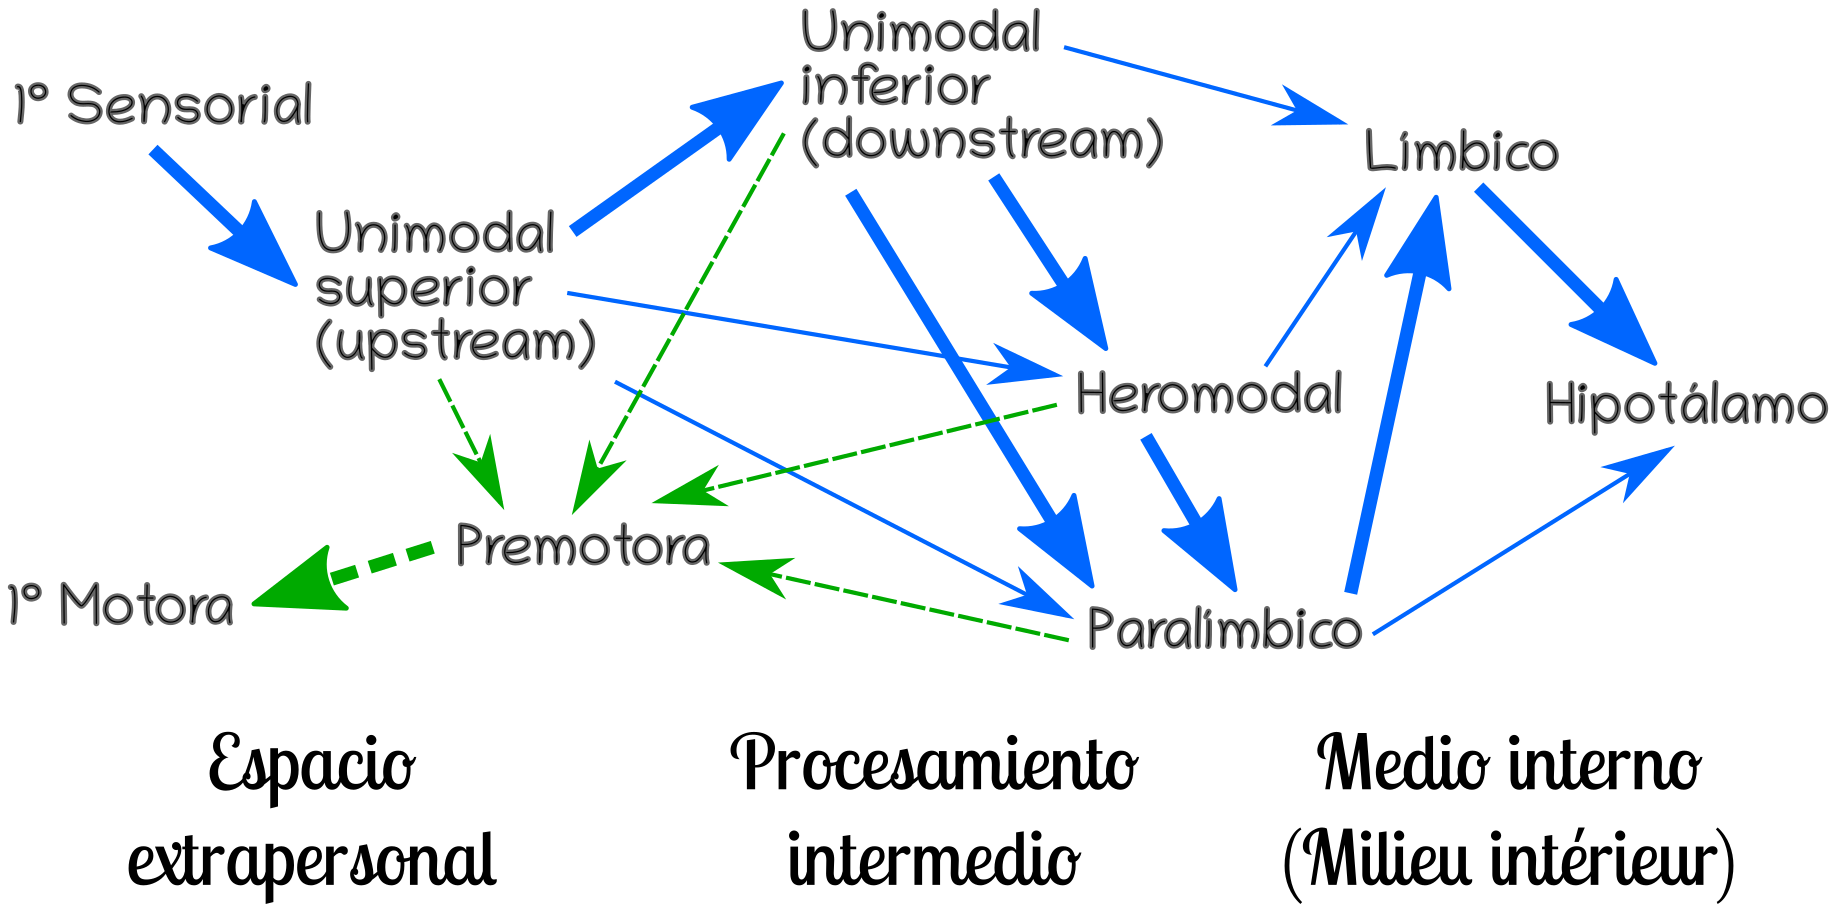
\includegraphics[width=0.9\textwidth]{../Figuras/zonasFuncionales.png}
  \caption{Diagrama de la arquitectura del cerebro a nivel funcional. Enfocado en sentido de la visión o la audición. \parencite{Mesulam1998}. Redibujado por Verónica E. Arriola Ríos. }
  \label{fig:zonasFun}
 \end{figure}

Explicación: El punto de partida de la ruta es la capa sensorial, que vamos a considerar como \textbf{la entrada}. El cerebro está recibiendo información en el momento que existe una señal que viene del mundo exterior.

Su primera conexión es hacia la capa unimodal superior, que vamos a considerar como \textbf{la primera capa}, donde se procesa la información más básica de la señal (del sentido), tales como el color, las formas o los tonos de sonido.

Luego están las capas intermedias unimodal inferior, heteromodal, paralímbico, límbico, donde se dará un procesamiento intermedio; se juntarán varias características interpretadas por la primera capa. Conforme avance la señal a las siguientes capas, las neuronas notarán características más complejas. 

En la capa unimodal y heteromodal se espera que la información codificada sea la percepción y una planeación motora. Es decir, que se va a formar el plan de reacción motora ante la señal. 

En las capas paralímbicas se espera que la información codificada sea el cambio de emoción y motivación. Es decir, que no habrá una reacción hacia el mundo solo hacia el pensamiento/cerebro y este refuerzo de señales hará un refuerzo/cambio de conducta a largo plazo.

En las capas límbicas se espera que se codifique la regulación de: la emoción, la motivación y memoria.

Una vez llege la señal con la codificación de todas las capas por las que paso al hipotálamo, este se encarga de coordinar las respuestas codificadas. Ya sea hacia la capa premotora o paralímbica. En el caso del diagrama las flechas en color verde indican que hubo una respuesta hacia la capa premotora, que tendrá una salida hacia los nervios motores, es decir una reacción motora inmediata de la señal. 


Cabe destacar que, si bien no es imprescindible contar con un conocimiento profundo del cerebro para trabajar con Redes Neuronales Artificiales (RNA), poseer una comprensión básica de las zonas funcionales del cerebro resulta fundamental para contextualizar problemas en el campo de la inteligencia artificial. Un ejemplo concreto es la comprensión del procesamiento del lenguaje en el cerebro, conocimiento usado para el desarrollo de aplicaciones de Procesamiento del Lenguaje Natural (PLN).

Esta atención especial a las zonas funcionales del cerebro se justifica por la necesidad de entender los conceptos fundamentales de entradas, capas, salidas y conexiones, los cuales son la base para comprender conceptos más avanzados como memoria y reacciones, tanto inmediatas como a largo plazo. Estos últimos conceptos son especialmente relevantes en modelos específicos, como las RNA de memoria a corto y largo plazo (LSTM, por sus siglas en inglés Long Short Time Memory) y las RNA con Unidad Recurrente con Puertas (GRU, por sus siglas en inglés Gate Recurrent Unit)  que se estudiarán detenidamente en etapas posteriores del curso.







